\documentclass[11pt]{article}

\usepackage[margin=1in]{geometry}
\usepackage{graphicx}
\usepackage{booktabs}
\usepackage{amsmath}
\usepackage{caption}
\usepackage{subcaption}
\usepackage{xcolor}
\usepackage[colorlinks=true,linkcolor=black,citecolor=black,urlcolor=blue]{hyperref}
\usepackage{microtype}
\usepackage{enumitem}

\graphicspath{{../figures/}}
\captionsetup{font=small,labelfont=bf}
\setlist{itemsep=2pt,parsep=0pt,topsep=4pt}

\newcommand{\qual}[1]{\textsf{#1}}
\newcommand{\claim}[1]{\vspace{-7pt}\par{\small\itshape #1}\par\vspace{3pt}}

\title{\bfseries Teaching Quality Is Linearly Decodable}
\author{Sophia Zhang}
\date{August 2026}

\begin{document}
\maketitle

\section*{Summary}

RL for tutoring needs a per-turn reward for teaching quality. LLM-as-judge is accurate but far too
slow to sit inside a training loop. We fit a ridge regression from a frozen OLMo-2-7B-Instruct's
mid-layer activations to human ratings of a tutor turn, and use it as the reward for GRPO. It costs
one dot product per turn.

\begin{itemize}
\item \textbf{Outcome-based rewards cannot work, measurably.} Rated teaching quality correlates with
the simulated student solving at $r=-0.012$; rated answer-leakage at $+0.291$. Student outcome carries
one signal, and the only lever a tutor has on it is giving the answer away.
\item \textbf{The probe's claim survives a blind check.} It claimed $+0.36$ over the untrained policy
on 60 held-out questions; a human rater and a panel of six models, neither able to see the scores or
which policy wrote which turn, paid $+0.34$ and $+0.35$.
\item \textbf{Three failures the reward curve could not show.} Turns collapsed toward brevity (12\%
rated too short $\rightarrow$ 29\%). One arm claimed half again more than it was paid. And an arm that
fixed the length problem was ranked \emph{worse} by both automated judges while the human preferred it
29--11, because both tie leakage to length about 1.6$\times$ as strongly as she does.
\item \textbf{The reward model is the ceiling, not the optimiser.} Across seven arms, learning rates
spanning 4$\times$ converge to the same reward. Capability is untouched: $-0.3$ points pooled over
ARC-Challenge, MMLU stem and GSM8K.
\end{itemize}

\begin{figure}[h]
\centering
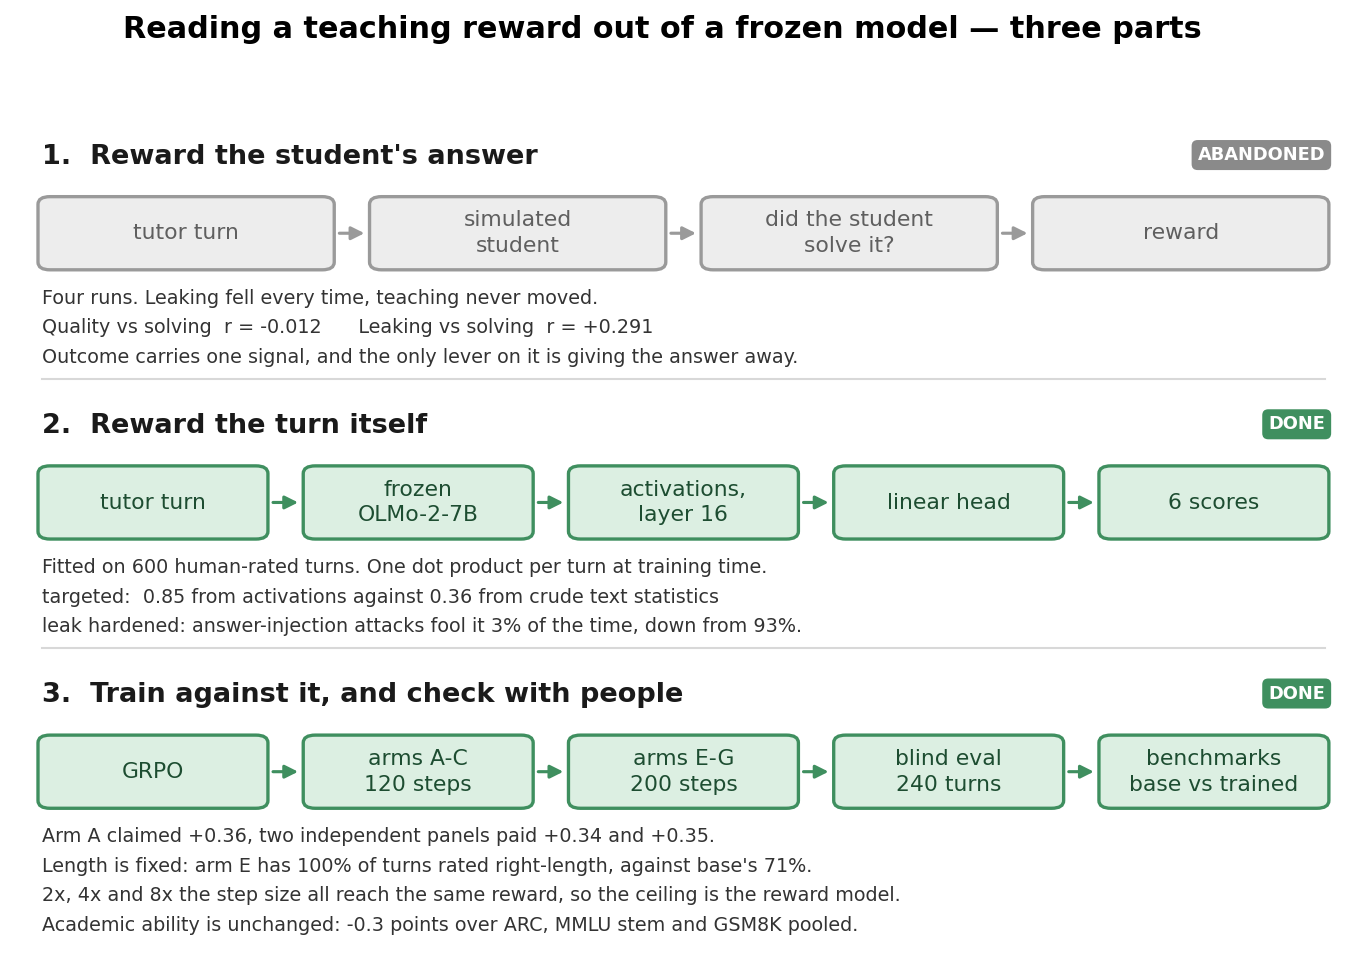
\includegraphics[width=\textwidth]{overview.png}
\caption{The three parts of the project. The first is a dead end, drawn because it is why the reward
reads the tutor's turn rather than the student's outcome, and because it cost four training runs to
establish.}
\label{fig:overview}
\end{figure}

\begin{figure}[p]
\centering
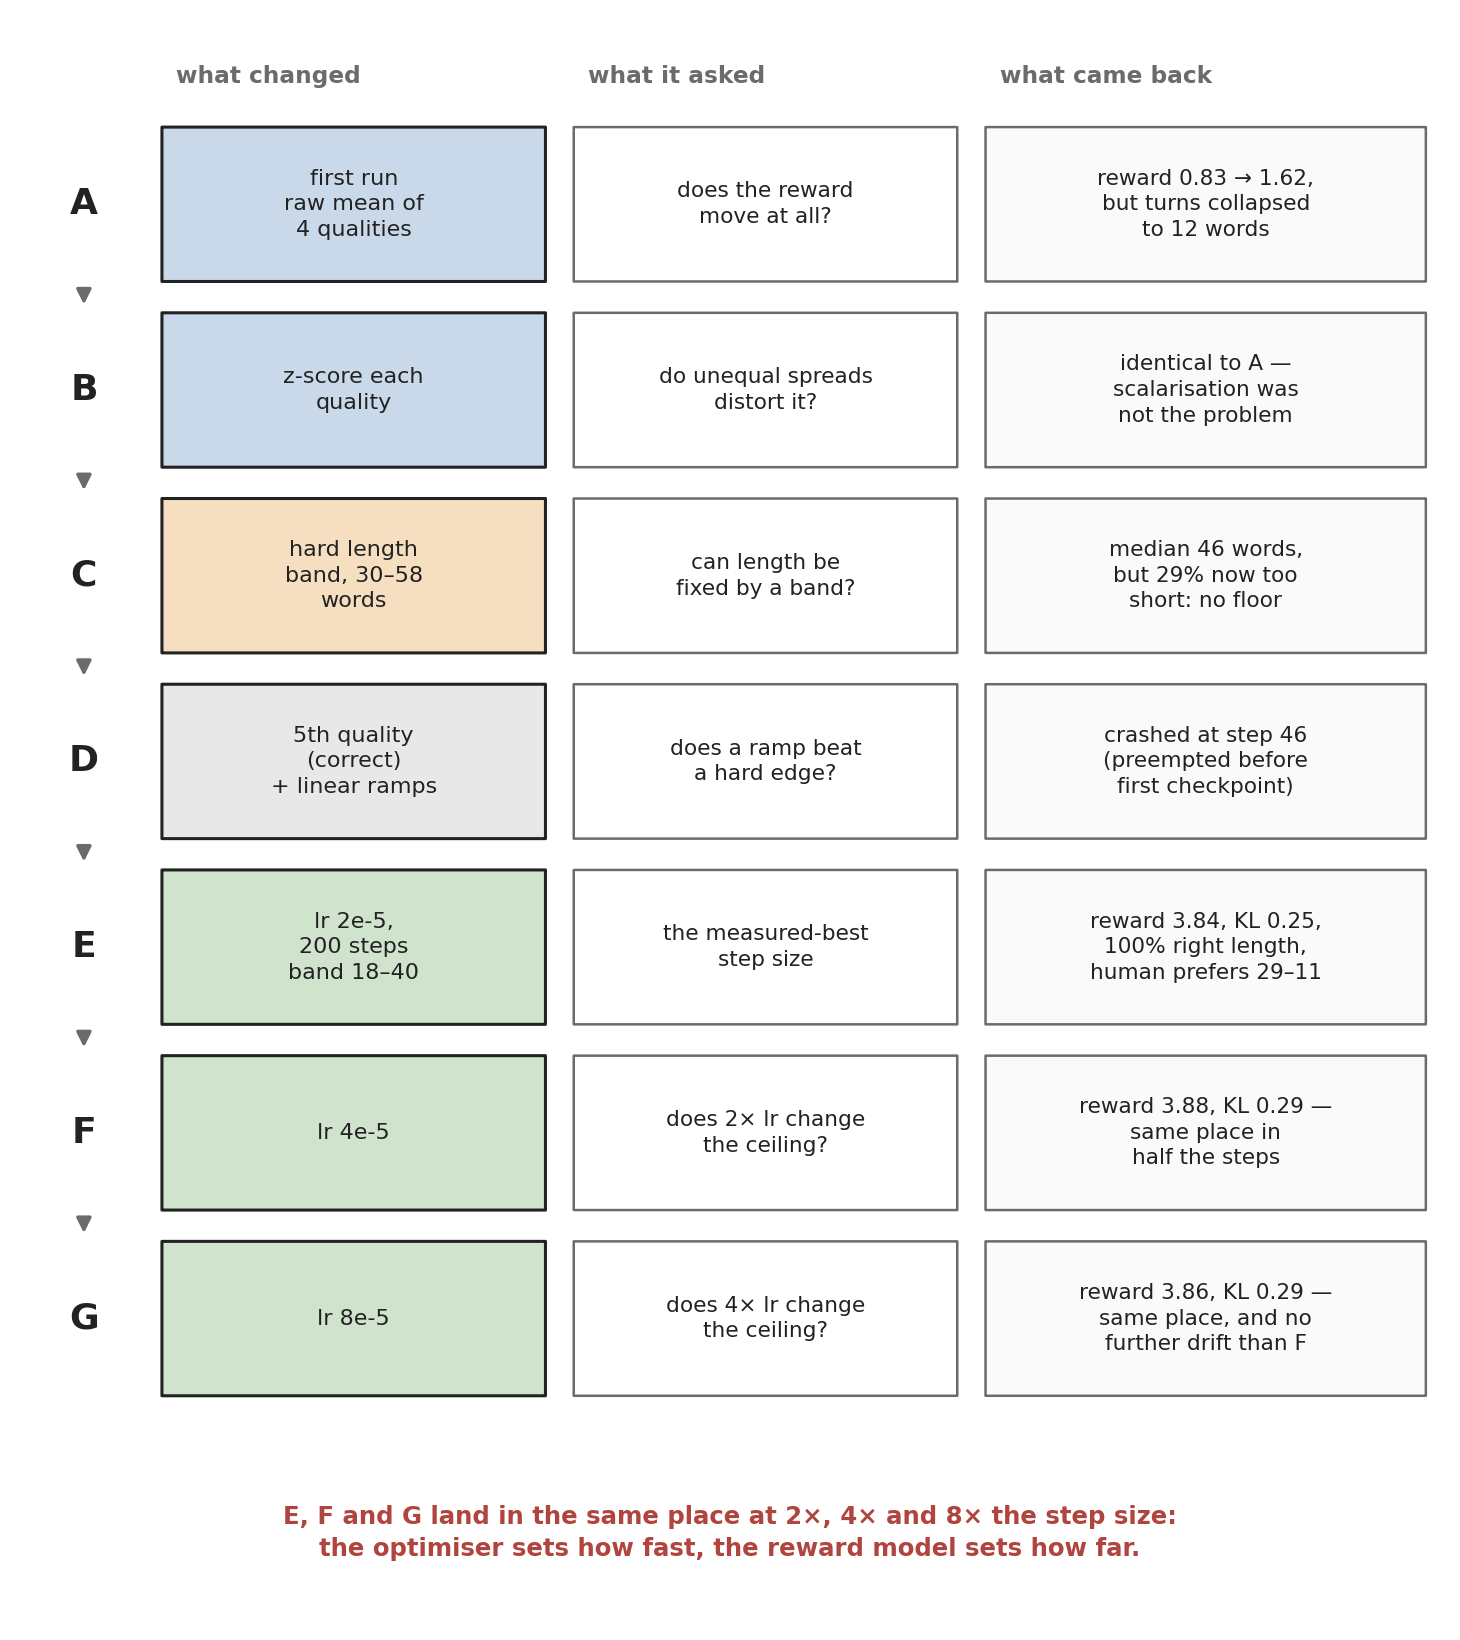
\includegraphics[width=\textwidth]{ablations.png}
\caption{Every arm: what it changed, what it asked, what came back. The arms were sequential, each
designed after reading the last. A and B show the scalarisation was not the problem; C and D are about
length; E, F and G vary only the learning rate.}
\label{fig:ablations}
\end{figure}

\section{The Data}
\label{sec:data}
\claim{Released US state exam items, with dialogues generated on them by two off-the-shelf models.}

\paragraph{Questions.} 307 released multiple-choice items from public-school standardised tests in
five US states --- California, Pennsylvania, Massachusetts, New Jersey, Texas --- published 2001--2026.
Four options each with a known key. Grades 3--11, modal grade 8; roughly 40\% mathematics, 32\%
science, 28\% social studies. Chosen because the correct answer is externally given, so nothing has to
be adjudicated, and because they are what school students are actually set.

\paragraph{Dialogues.} 299 of those items generated 1200 tutor--student conversations: 3600 tutor
turns and 4800 student turns, three tutor turns each. Tutor is OLMo-2-7B-Instruct, the model later
trained; student is Qwen-2.5-1.5B-Instruct prompted to work the problem and err plausibly. Four tutor
prompt styles in equal share --- \emph{brief}, \emph{socratic}, \emph{plain}, \emph{explain} --- so the
corpus spans a range of teaching behaviour rather than one house style.

\paragraph{Ratings and splits.} 600 tutor turns were sampled and rated by hand and by models; this is
what the probe is fitted on. Questions split 250 train / 50 evaluation with no overlap. Each
(question, dialogue-so-far) pair is one prompt, giving 1000 training and 200 evaluation prompts.

\section{Why Not Reward the Student's Answer}
\label{sec:why}
\claim{Student outcome carries one signal, and answer-leakage is the only lever on it.}

Four GRPO runs rewarded the tutor when a simulated student subsequently solved the problem, across two
reward formulations, two corpora, and a corrected leak detector. All four taught the tutor to stop
giving answers away; none improved held-out teaching.

\begin{table}[h]
\centering
\begin{tabular}{lr}
\toprule
\textbf{Property of the tutor turn} & \textbf{Correlation with the student solving} \\
\midrule
Rated tutoring \emph{quality} & $-0.012$ \\
Rated \emph{answer leakage}   & $+0.291$ \\
\bottomrule
\end{tabular}
\caption{The best-rated turns had the worst solve rates.}
\label{tab:why}
\end{table}

Table~\ref{tab:why} is the cause. Outcome carries one signal --- whether the student was told the
answer --- so penalising leakage does not add a pedagogical signal, it removes the only one present.
Leak rate duly fell in every run while held-out teaching never moved.

\paragraph{The simulated student is trapped between two failures with nothing between them.} A weak
student \emph{cannot} learn: expert tutoring moved a 0.5B student's answers by roughly 7 percentage
points, which upper-bounds anything a reward computed from its accuracy could detect. A strong student
\emph{already knows the answer}: told to act confused, its chain of thought solves the problem anyway,
or it drops the persona and explains like the teacher. Filtering to harder items tightens the trap,
since items a weak student fails are those a strong model gets unaided. A 3B model in between was tried
and abandoned.

Two reward-side remedies also failed. A dense learned quality score turned out to detect \emph{which
model wrote the turn}, and drove question-asking from 79\% to 32\%. Removing the leak detector's false
positives more than doubled its precision on mathematics and moved the held-out measure by 0.008.

The premise of everything following: the measured quantity must admit a pedagogical channel before a
reward built on it can find one. We discard the student and rate the turn.

\section{The Reward Model}
\label{sec:probe}
\claim{A ridge fit on frozen mid-layer activations reads teaching quality where surface features cannot.}

Six qualities of a turn are rated 1--3 by humans: how much it \qual{leaks} the answer, how
\qual{targeted} to this student's error, how \qual{actionable}, how much it \qual{elicits} the
student's reasoning, whether its \qual{length} fits, and whether anything is in\qual{correct}. A ridge
regression predicts each from the frozen encoder's activations at a middle layer.

\begin{figure}[h]
\centering
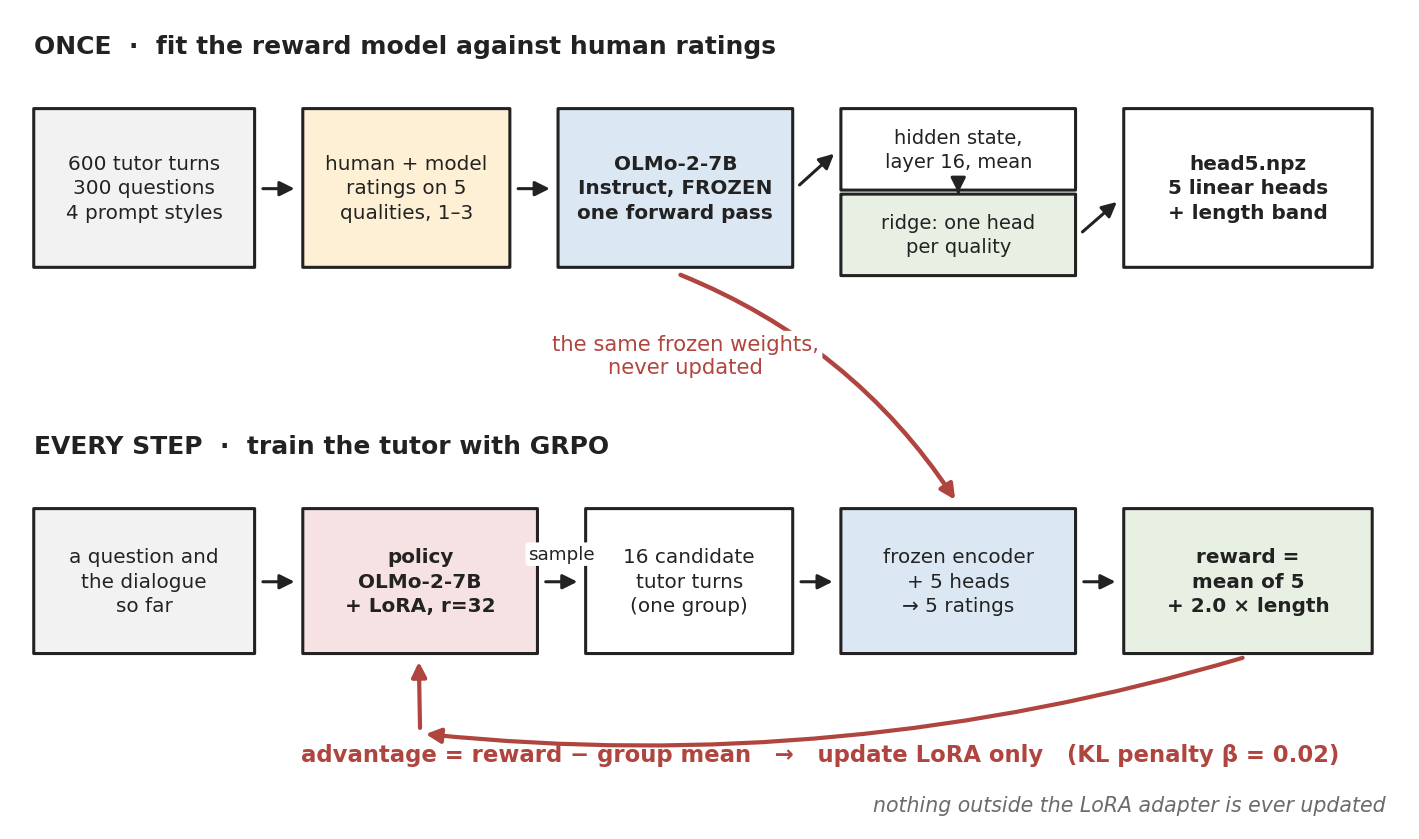
\includegraphics[width=\textwidth]{system.png}
\caption{The probe is fitted once, then called on every rollout. The encoder appears twice and is the
same frozen weights both times: the policy cannot raise its own score by moving its internal
representations, because the representations being read are not its own. Only the LoRA adapter is
updated.}
\label{fig:system}
\end{figure}

\begin{figure}[h]
\centering
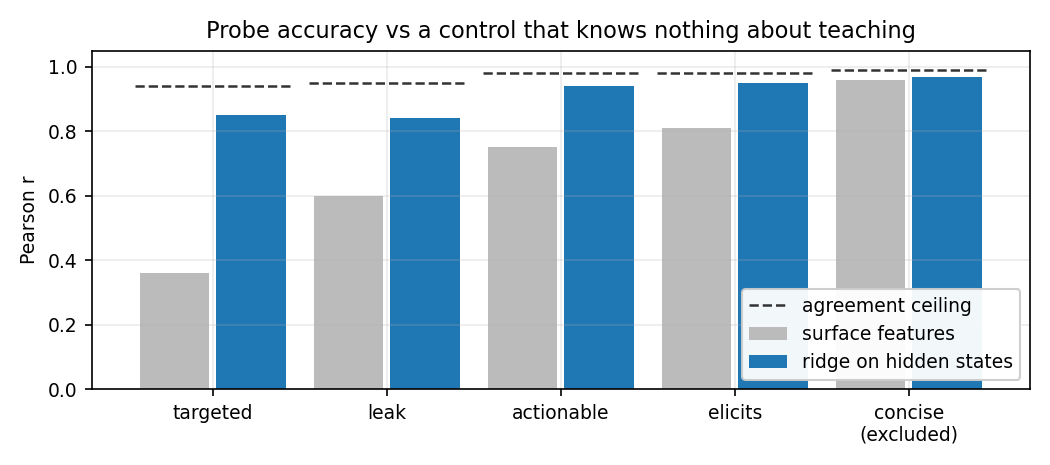
\includegraphics[width=0.86\textwidth]{probe_accuracy.png}
\caption{Probe accuracy against a control. Grey is eight surface features --- word count, question
marks, digit density --- that encode nothing about teaching. Where grey reaches blue, the rating is a
property of the text's shape and the activations bought nothing.}
\label{fig:probe}
\end{figure}

The control in Figure~\ref{fig:probe} is load-bearing. \qual{concise} is predicted at 0.96 by word
count against 0.97 from activations --- a word counter wearing a rubric, excluded from the reward.
\qual{targeted} is the opposite: 0.36 from surface features against \textbf{0.85} from activations.
Whether a turn addresses the student's actual mistake is nearly invisible in surface form, and the
model tracks it anyway.

Ridge beat a PCA-fronted, separately tuned MLP on every quality, so the map is effectively linear.
Layers 16--20 of 32 beat both ends; the final layer is occupied predicting the next token rather than
summarising the turn.

\paragraph{Hardening against the obvious attack.} Injecting the gold answer into an otherwise
withholding turn fooled the first leak head 93\% of the time; after adversarial training, \textbf{3\%},
including on phrasings and insertion points never fitted on, with accuracy on genuine turns holding at
0.84 $\rightarrow$ 0.82. The fitting script refuses to emit a head missing more than 15\% of held-out
attacks.

\section{Training Setup}
\label{sec:setup}
\claim{GRPO on OLMo-2-7B-Instruct with LoRA, $r=32$, on one GPU.}

GRPO samples 8 candidate turns per prompt and moves the policy toward those scoring above their group
mean. Only a LoRA adapter at $r=32$ is trained; the 7B base is frozen. Throughout we report KL
divergence from the initial policy (``drift'', in nats), because a reward can always be raised by
moving further, so a gain is only interesting per unit of distance travelled. The two first-round arms
differ only in scalarisation.

\begin{table}[h]
\centering
\begin{tabular}{lll}
\toprule
& \textbf{Arm A} & \textbf{Arm B} \\
\midrule
Scalarisation & plain average & each score z-scored, then averaged \\
Hardware & 1$\times$H100 & 1$\times$H200 \\
\bottomrule
\end{tabular}
\caption{The two first-round arms.}
\label{tab:arms}
\end{table}

Arm B exists because a plain average weights each quality by how much it happens to vary.
\qual{elicits} varies most and \qual{targeted} least, so a plain average leans $1.5\times$ harder on
the quality surface features already predict at 0.81 than on the one they predict at 0.36 --- backwards
for this project.

\section{Training Results}
\label{sec:training}
\claim{Reward rises, generalises to held-out questions, and length falls throughout.}

Reward rises 1.45 $\rightarrow$ 1.63 and rises as much on the 50 held-out questions as on the 250
trained on. Length falls throughout: arm A 38 $\rightarrow$ 27 words, arm B 43 $\rightarrow$ 23. Arm
B's scalar sits at zero by construction, since z-scoring centres it, so arm B must be read through its
individual qualities.

Three of four rewarded qualities improve by 0.25--0.40 points. \qual{targeted} is flat in both arms, a
property of the labels rather than the training: the untrained policy already scores 2.58 of 3, and a
linear fit on ratings that lopsided hedges to the middle and never predicts a full 3.

\paragraph{Is 1.6 high?} Against the corpus the probe was fitted on, 1.60 is the 78th percentile and
below the mean of the best prompt style --- so the policy is scored \emph{inside} the range the fit
learned from rather than off its end. That stops holding above roughly 1.8, which arm A approaches.

\section{Blind Evaluation}
\label{sec:blind}
\claim{The probe claimed $+0.36$; two independent panels paid $+0.34$ and $+0.35$.}

The predecessor project's reward improved for four consecutive runs while the quantity it stood for
never moved, so a rising curve is not evidence. Sixty held-out questions were answered by three
policies --- untrained, arm A, arm B --- giving 180 turns with policy identity and scores stripped and
identifiers salted. One human rated 51 turns and judged 47 pairs. Six frontier models rated all 180
after calibration on 26 of her ratings and \emph{validation against 25 they were never shown}. Every
policy answered the same questions, holding difficulty and student state fixed.

\subsection{Claimed against paid}

\begin{table}[h]
\centering
\begin{tabular}{lrrrrr}
\toprule
\textbf{Who is measuring} & \textbf{Untrained} & \textbf{Arm A} & \textbf{Arm B}
& \textbf{Gain, A} & \textbf{Gain, B} \\
\midrule
Model raters, 180 turns & 1.32 & 1.65 & 1.71 & $+0.34$ & $+0.40$ \\
Human, 51 turns         & 1.31 & 1.66 & 1.68 & $+0.35$ & $+0.37$ \\
\textbf{Reward model}   & 1.23 & 1.60 & 1.72 & $\mathbf{+0.36}$ & $\mathbf{+0.49}$ \\
\bottomrule
\end{tabular}
\caption{Claimed gain against paid gain. Absolute levels are not comparable across rows; the gain is.}
\label{tab:gain}
\end{table}

\textbf{Arm A is clean}: claimed $+0.36$, paid $+0.34$ and $+0.35$. That three-way agreement is the
strongest evidence the training did something real rather than exploiting the scorer.

\textbf{Arm B is where a gap opens}: claimed $+0.49$, paid $+0.37$ and $+0.40$. Mild, but it is the
shape of a policy optimising the scorer rather than the quantity it represents, and it appears in the
arm that optimised harder. The spread of reward across turns also collapses from 0.36 untrained to 0.18
and 0.13 --- a policy settling into one shape of answer.

\subsection{Which qualities moved}

\begin{figure}[h]
\centering
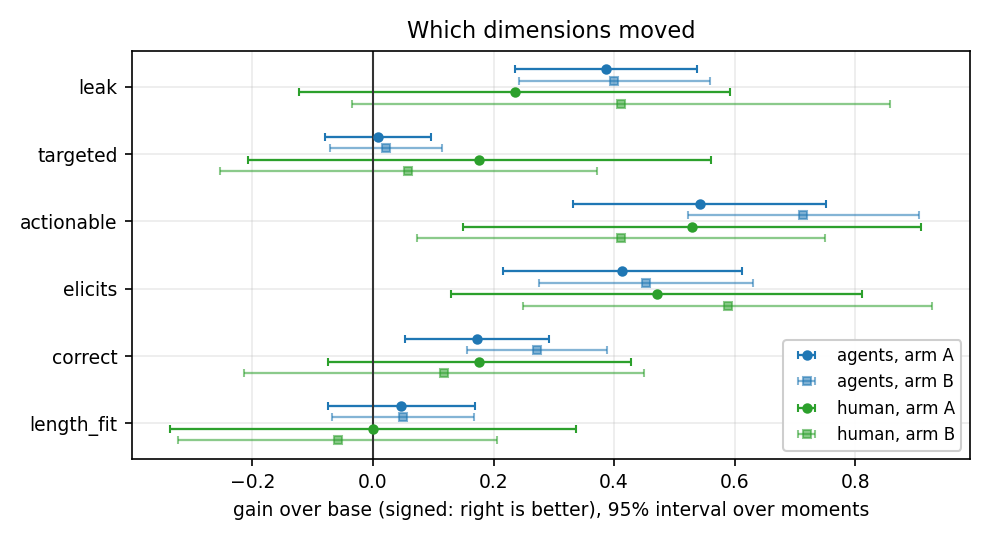
\includegraphics[width=0.92\textwidth]{dimension_gaps.png}
\caption{Gain over untrained, signed so right is always better, with 95\% intervals over questions. The
human's intervals are wider throughout: 17 questions against 60.}
\label{fig:dims}
\end{figure}

\begin{table}[h]
\centering
\begin{tabular}{lrrlr}
\toprule
\textbf{Quality} & \textbf{Arm A} & \textbf{Arm B} & \textbf{Human, A / B}
& \shortstack{\textbf{Raters match}\\\textbf{human, per turn}} \\
\midrule
\qual{leak}        & $\mathbf{+0.39}$ (69\%) & $\mathbf{+0.40}$ (72\%) & $+0.24$ / $+0.41$ & 0.37 \\
\qual{actionable}  & $\mathbf{+0.54}$ (69\%) & $\mathbf{+0.71}$ (82\%) & $\mathbf{+0.53}$ / $\mathbf{+0.41}$ & 0.03 \\
\qual{elicits}     & $\mathbf{+0.41}$ (64\%) & $\mathbf{+0.45}$ (70\%) & $\mathbf{+0.47}$ / $\mathbf{+0.59}$ & 0.21 \\
\qual{correct}     & $\mathbf{+0.17}$ (65\%) & $\mathbf{+0.27}$ (73\%) & $+0.18$ / $+0.12$ & 0.38 \\
\qual{targeted}    & $+0.01$ & $+0.02$ & $+0.18$ / $+0.06$ & 0.24 \\
\qual{length\_fit} & $+0.05$ & $+0.05$ & $+0.00$ / $-0.06$ & 0.26 \\
\bottomrule
\end{tabular}
\caption{Bold exceeds its margin of error. Percentages are the share of questions won. The last column
runs 0 (chance) to 1 (perfect).}
\label{tab:dims}
\end{table}

\paragraph{Disagreeing per turn and agreeing per policy are different measurements.} On
\qual{actionable} the model raters match the human at 0.03 --- chance at ranking one turn against
another --- yet both panels produce the same gap between policies, same direction and nearly the same
magnitude ($+0.54/+0.71$ against $+0.53/+0.41$). Ranking noise cancels across sixty questions; a
consistent preference does not. Near-zero per-turn agreement therefore disqualifies these raters for
\emph{labelling training data} and says little about \emph{comparing policies}. Conflating the two would
have discarded this evaluation's main result.

\subsection{The regression the reward curve could not show}

\begin{table}[h]
\centering
\begin{tabular}{lrrr}
\toprule
& \textbf{Too short} & \textbf{Right} & \textbf{Too long} \\
\midrule
Untrained & 12\% & 71\% & 18\% \\
Arm A     & \textbf{29\%} & 71\% & 0\% \\
Arm B     & \textbf{35\%} & 65\% & 0\% \\
\bottomrule
\end{tabular}
\caption{Human length judgements. Training eliminated over-long turns and paid triple the too-short
rate, leaving the mean flat.}
\label{tab:length}
\end{table}

\qual{length\_fit} scores 2 for right and 1 or 3 for the two ways of being wrong, so its mean hides an
even split --- a policy divided evenly between the two failures averages exactly ideal. The model raters
put too-short at 20\% and 15\%, about half the true figure: the one place where trusting them alone
would have hidden a real loss.

\subsection{Head-to-head preferences}

\begin{table}[h]
\centering
\begin{tabular}{lccc}
\toprule
\textbf{Comparison} & \textbf{Result} & \shortstack{\textbf{Probability}\\\textbf{by chance}}
& \shortstack{\textbf{Agreed with}\\\textbf{reward model}} \\
\midrule
Arm A vs.\ arm B, 17 pairs      & 8--9, no ties & 100\% & 47\% \\
Arm A vs.\ untrained, 30 pairs  & \textbf{18--10}, 2 ties & 19\% & \textbf{68\%} \\
\bottomrule
\end{tabular}
\caption{Blind pairwise preferences, same question on both sides.}
\label{tab:pref}
\end{table}

The two arms are indistinguishable to a person. Against untrained, training wins 64\% of decided pairs
--- right direction, but 28 decided pairs cannot rule out chance where a 64\% effect needs roughly 60.
With the absolute ratings, which rest on far more judgements and put arm A ahead on 76\% of questions,
we conclude training beat the untrained policy.

The final column is more informative: the reward model \emph{cannot} separate two trained policies
(47\%, scoring the two sides within 0.07) but \emph{can} separate trained from untrained (68\%). Real
but coarse resolution is the honest characterisation.

\subsection{Why the model ratings were not used to refit the probe}

\begin{figure}[h]
\centering
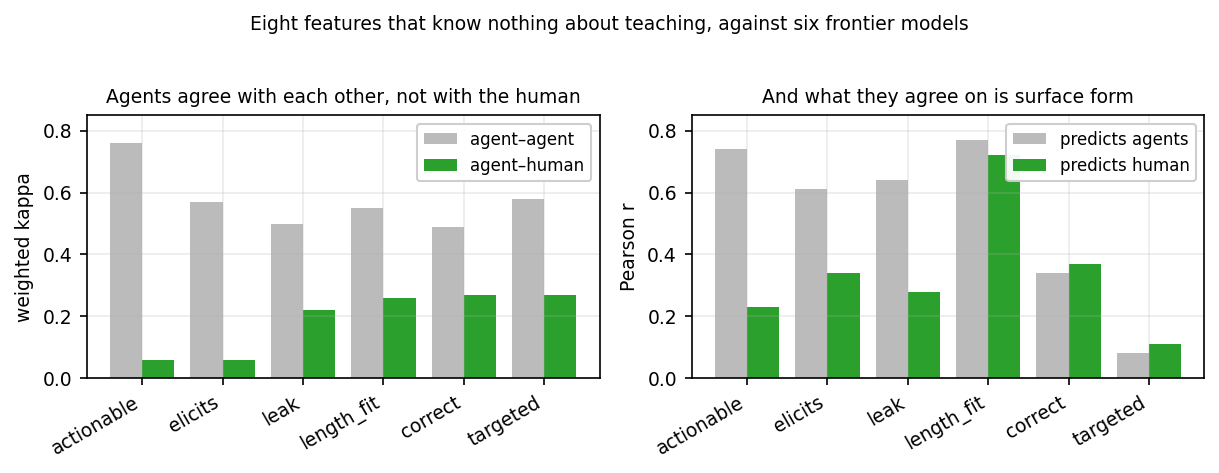
\includegraphics[width=0.98\textwidth]{agent_trust.png}
\caption{Left: the six raters agree with each other far more than with the human they were calibrated
to. Right: what they agree on is largely surface form.}
\label{fig:trust}
\end{figure}

The shortcut is to treat six frontier models as a cheap annotation panel. Figure~\ref{fig:trust} is why
we did not: on \qual{actionable} they agree with each other at 0.76 and with the human at 0.06, and
three quarters of their consensus is reproducible from eight surface features. Refitting on that would
optimise surface form --- the length collapse just measured. Only \qual{correct} and \qual{targeted} are
not surface-driven, and only those two are safe to average.

Low per-turn agreement also has a benign cause: little room to disagree. \qual{actionable} is rated 3 on
74\% of turns by the models and 65\% by the human, so everyone is choosing between 2 and 3. The score
\emph{distributions} match on all six qualities, differing only in which turn gets which --- the regime
where averaged model ratings are trustworthy for comparing policies and untrustworthy for labelling
single turns.

\section{Ablation Results}
\label{sec:round2}
\claim{A rebuilt rubric, a measured learning rate, two failed repairs, and a ceiling belonging to the reward model.}

The blind evaluation left three things to repair: one clear success, one measurement that changed a
default, and two failures worth reporting as failures.

\subsection{The rubric was measuring fewer things than it claimed}

Three properties of the original labels, none arguable:

\begin{itemize}
\item \qual{actionable} and \qual{elicits} correlate at \textbf{0.95}: one quality with two names,
counted twice.
\item The five qualities have effective rank \textbf{2.9}; the first principal component explains 47\%
of the variance.
\item Nine turns are top-quartile on \qual{leak}, \qual{targeted}, \qual{actionable} \emph{and}
\qual{elicits} at once, median length \textbf{12 words} against a corpus median of 30.
\end{itemize}

That last item is the length collapse, visible in the labels before any training. A short bare question
satisfies four of five qualities simultaneously, so the reward had a degenerate optimum and RL found it.

The cause is structural: every original quality measures what the tutor \emph{withheld} --- didn't
reveal, didn't over-explain, left the thinking to the student --- and none measures what it
\emph{contributed}. A rubric of withholding measures is maximised by maximal withholding. Across 70
effect sizes, elaborated feedback is $d=0.49$, knowledge of the correct response $d=0.32$, bare
knowledge of results $d=0.05$. The reward was maximising the $d=0.05$ end.

\begin{figure}[h]
\centering
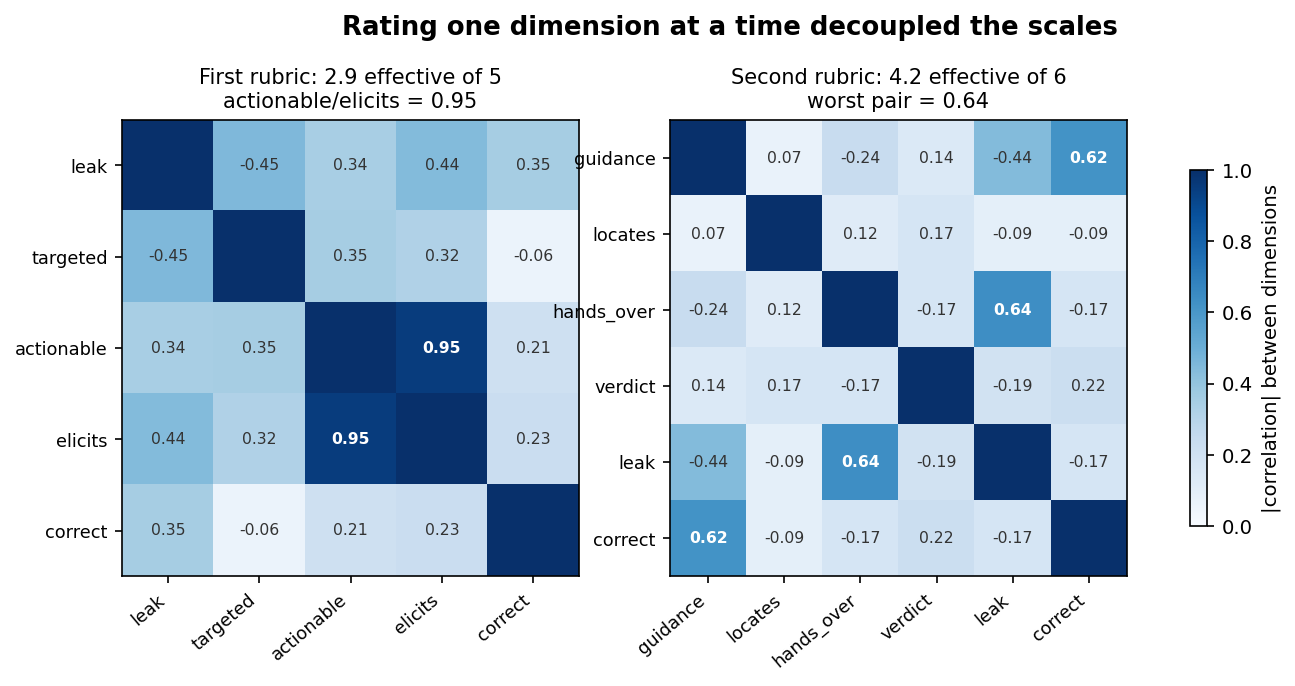
\includegraphics[width=\textwidth]{decoupling.png}
\caption{Absolute correlations between qualities. Rating one quality at a time across all turns, rather
than six per turn, breaks the coupling that made \qual{actionable} and \qual{elicits} one measurement.}
\label{fig:decoupling}
\end{figure}

\subsection{The replacement, and how much better raters agree on it}

Six qualities replace the six: \qual{guidance} (does the turn supply anything usable), \qual{locates}
(does it point at something specific in the student's message), \qual{hands\_over} (does it hand over
the next move and name it), \qual{verdict} (does its right/wrong signal match what the student said),
\qual{leak}, \qual{correct}. A seventh, \qual{student\_state}, is rated on the \emph{student's} message
and never enters the reward; it exists so contingency can be computed later. Five models rated 44 turns,
one full pass per quality so judging one could not colour the next.

\begin{table}[h]
\centering
\begin{tabular}{lrrl}
\toprule
\textbf{Quality} & \textbf{Weighted $\kappa$} & \textbf{Ceiling} & \textbf{Replaces} \\
\midrule
\qual{leak}        & \textbf{0.83} & 0.93 & same wording; was 0.51 \\
\qual{hands\_over} & \textbf{0.81} & 0.93 & \qual{elicits}, which was 0.56 \\
\qual{correct}     & \textbf{0.80} & 0.93 & same construct, reference solution now shown; was 0.18 \\
\qual{verdict}     & 0.73 & 0.86 & new \\
\qual{locates}     & 0.67 & 0.83 & \qual{targeted}, which was 0.57 \\
\qual{guidance}    & 0.51 & 0.74 & new, and the weakest \\
\bottomrule
\end{tabular}
\caption{Inter-rater agreement across five raters. All six clear the 0.4 threshold; two of the original
six did not.}
\label{tab:v2}
\end{table}

Two results beat the averages. \qual{hands\_over} scores 0.81 where \qual{elicits} scored 0.56, and the
only change is framing: ``does the turn hand over the next move'' rather than ``how much thinking does it
ask for.'' The literature predicted this --- behavioural framings of the construct reach $\kappa$
0.55--0.95, cognitive-demand framings 0.09--0.34. And \qual{correct} went 0.18 $\rightarrow$ 0.80 through
an interface change, not a rewording: raters had been re-deriving the mathematics, and are now shown a
generated worked solution to check against.

\subsection{The reward is largely a length penalty, and the new rubric does not fix that}

Agreement was the wrong property to check alone. What the dimensions correlate \emph{with} explains
more of this project's history than what raters agree on. Running the head over all 600 labelled turns,
against the seven-rater consensus on the same turns:

\begin{table}[h]
\centering
\begin{tabular}{lrr}
\toprule
& \textbf{Probe} & \textbf{Labels} \\
\midrule
\qual{actionable} $\leftrightarrow$ \qual{elicits} & \textbf{0.96} & \textbf{0.95} \\
\qual{leak} $\leftrightarrow$ $\log$(words) & $+0.64$ & $+0.53$ \\
\qual{correct} $\leftrightarrow$ $\log$(words) & $-0.58$ & $-0.43$ \\
\qual{elicits} $\leftrightarrow$ $\log$(words) & $-0.52$ & $-0.50$ \\
\qual{actionable} $\leftrightarrow$ $\log$(words) & $-0.42$ & $-0.40$ \\
\qual{targeted} $\leftrightarrow$ $\log$(words) & $\mathbf{+0.03}$ & $\mathbf{+0.02}$ \\
\midrule
mean $|r|$ among the five & 0.43 & 0.37 \\
first principal component & 51\% & 47\% \\
effective rank & 3.07 / 5 & 3.31 / 5 \\
\bottomrule
\end{tabular}
\caption{The probe amplifies the label structure and invents none of it: every correlation matches the
labels in sign and exceeds it by 0.01--0.15. The redundancy is a property of the ratings.}
\label{tab:corr}
\end{table}

Applying the reward signs resolves the picture. \qual{leak} is negated, so its $+0.64$ becomes $-0.64$
and joins the other three: \qual{correct} $-0.58$, \qual{elicits} $-0.52$, \qual{actionable} $-0.42$,
with \qual{targeted} alone at $+0.03$. \textbf{The composite reward correlates with length at $-0.60$
in the probe and $-0.57$ in the labels.}

That is not a side effect but most of what the reward is, and it accounts for the sequence rather than
sitting alongside it: why arm A collapsed to 12 words, why a length term had to be introduced, why that
term supplies roughly 70\% of the measured gain --- it is the only one pushing back --- and why the
probe dimensions collected only 40\% of their available headroom, the remainder lying behind the
collapse the band blocks. \qual{targeted} is the exception, and it is also where surface features do
worst (0.36 against 0.85); it is the one dimension length cannot fake and the one the policy improved
least on.

\paragraph{V2 fixes the redundancy and not the length coupling.} \qual{guidance} was included partly as
a length-\emph{positive} counterweight, so this is checkable: nine raters scored 44 turns on all six V2
dimensions. But 24 of those 44 are manufactured negatives, each corrupted along a single dimension,
which decorrelates the dimensions by construction and says nothing about the rubric. Excluding them
leaves 20 real turns.

\begin{table}[h]
\centering
\begin{tabular}{lrrr}
\toprule
& \textbf{V1 ($n$=600)} & \textbf{V2, all 44} & \textbf{V2, real only ($n$=20)} \\
\midrule
mean $|r|$ & 0.37 & 0.22 & 0.28 \\
max $|r|$ & \textbf{0.95} & 0.65 & 0.70 \\
first PC & 47\% & 36\% & 40\% \\
effective rank & 3.31 / 5 & 4.88 / 6 & \textbf{4.53 / 6} \\
composite vs $\log$(words) & \textbf{$-0.57$} & $-0.37$ & \textbf{$-0.62$} \\
\bottomrule
\end{tabular}
\caption{The last column is the one to read. V2 genuinely removes the redundancy --- the 0.95 duplicate
is gone and effective rank rises from 3.31 of 5 to 4.53 of 6 --- while the length coupling is
unchanged at $-0.62$ against V1's $-0.57$.}
\label{tab:v2corr}
\end{table}

Per dimension on real turns: \qual{correct} $-0.66$, \qual{verdict} $-0.53$, \qual{hands\_over}
$-0.51$, \qual{leak} $-0.26$, \qual{guidance} $-0.12$, \qual{locates} $-0.06$. The two dimensions
designed to be length-neutral are, and the other four swamp them; \qual{guidance} was meant to be
length-positive and came out neutral. At $n=20$ the interval on $-0.62$ is roughly $[-0.84, -0.24]$, so
this cannot show V2 is worse --- only that it does not help.

The conclusion is that rubric wording is the wrong lever here. Decorrelating the dimensions from each
other and decorrelating them from length are separate problems; V2 solves the first and leaves the
second untouched, because raters score shorter turns higher on most pedagogical qualities under either
rubric. Brevity is confounded with quality in their own judgements, so any head fitted on this corpus
inherits it. The lever is the corpus --- turns in which length and quality vary independently --- which
has now been identified as necessary twice and still does not exist.

\subsection{Negative examples had to be manufactured}

The pool contained almost no bad turns: in a 20-turn pilot \qual{locates} never received the bottom score
and \qual{guidance} received it once, and a head cannot learn an anchor from zero examples. Real turns
were corrupted along one quality each --- the trick that took answer-injection from 93\% to 3\% --- and
rated blind. Four of six recipes landed unanimously; \qual{guidance} and \qual{locates} landed half the
time, because ``strip out the content'' can be satisfied halfway. Restated as prohibitions --- not one
number or content word from the student's message may appear --- overlap with the student's own words fell
from 5.6 to 0.2 for \qual{locates}.

\paragraph{A methodological failure worth recording.} The corrupted turns' identifiers encoded which
quality had been corrupted. One rater read the answer off the identifier prefix rather than judging the
turn, and said so in its report; its labels were discarded and identifiers are now salted hashes. It
surfaced only because that rater described its method honestly, which is a thin thing to have relied on.

\subsection{The learning rate, measured rather than chosen}

Four 35-step runs, identical apart from the rate, compared on reward gained per unit of KL drift. Reward
alone ranks runs by learning rate and is uninformative; the ratio has an interior maximum.

\begin{table}[h]
\centering
\begin{tabular}{lrrrrr}
\toprule
\textbf{Rate} & \textbf{Reward gain} & \textbf{KL} & \textbf{Gain/KL} & \textbf{Words} & \textbf{In band} \\
\midrule
\textbf{2e-5} & $+0.526$ & 0.074 & \textbf{7.11} & 50$\rightarrow$40 & 0.90 \\
1e-5 & $+0.348$ & 0.080 & 4.35 & 50$\rightarrow$31 & 0.81 \\
4e-5 & $+0.526$ & 0.122 & 4.31 & 50$\rightarrow$43 & 0.92 \\
8e-5 & $+0.606$ & 0.172 & 3.52 & 49$\rightarrow$36 & 0.94 \\
\bottomrule
\end{tabular}
\caption{2e-5 buys the same gain as 4e-5 for 40\% less drift.}
\label{tab:lr}
\end{table}

The word-count column is the more interesting result: the \emph{slowest} rate produced the
\emph{shortest} turns, 31 words against 40, and the in-band share rose monotonically with the rate. At
1e-5 the probe's pull toward brevity still dominates and the policy sits at the band's lower edge; from
2e-5 up it reaches the band and stays.

\subsection{Two attempts to decouple \qual{leak} from length, both unsuccessful}

The probe ties leakage to length at $+0.70$ on policy-generated turns against the human's $+0.43$, and
that distortion made both automated judges rank arm C below arm A when the human preferred it 29--11.

\begin{figure}[h]
\centering
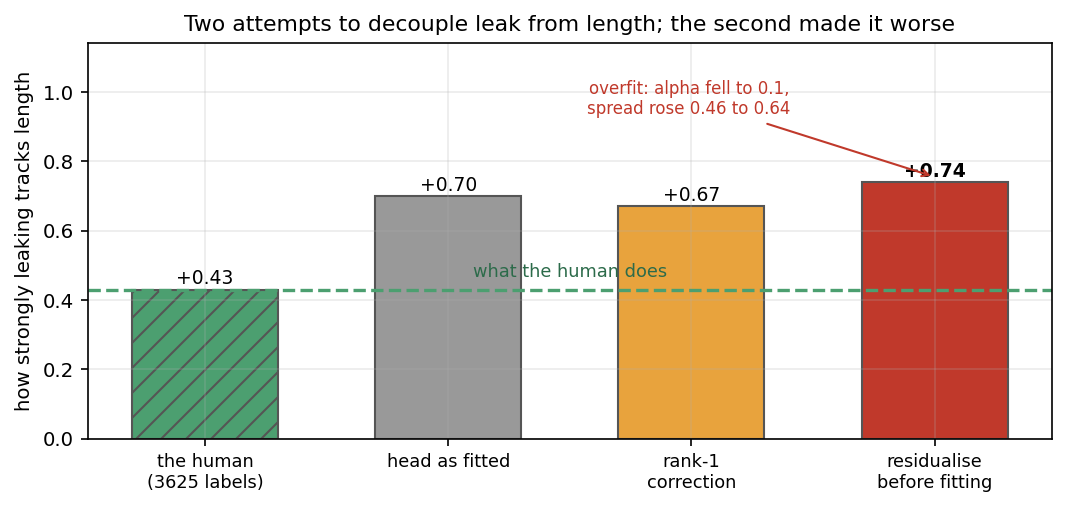
\includegraphics[width=0.86\textwidth]{leak_repairs.png}
\caption{A rank-1 correction toward the labels' own coupling achieved little; residualising length out of
both states and target before fitting made it worse.}
\label{fig:leakrepairs}
\end{figure}

The second attempt is the informative one. Residualising length out of the states should leave the head no
length direction to rediscover, and in-distribution it does. Out of distribution the coupling \emph{rose}
to $+0.74$, the ridge penalty collapsed to its smallest value, and prediction spread grew 0.46
$\rightarrow$ 0.64: the fit had begun memorising.

The diagnosis: in-distribution the head's coupling is 0.44 against the labels' 0.37, so there is almost
nothing to correct there. The $+0.70$ is distribution shift --- on policy-generated text the head has never
seen, length becomes a far stronger cue --- and no correction estimated in-distribution reaches a problem
that exists only out of it. Fixing it requires labels on policy-generated turns.

Until then the explicit length term is the only predictable lever, so it went from a hard band to a band
with linear ramps: a hard band scores 59 and 200 words identically, so nothing pushes a runaway turn back.

\begin{figure}[h]
\centering
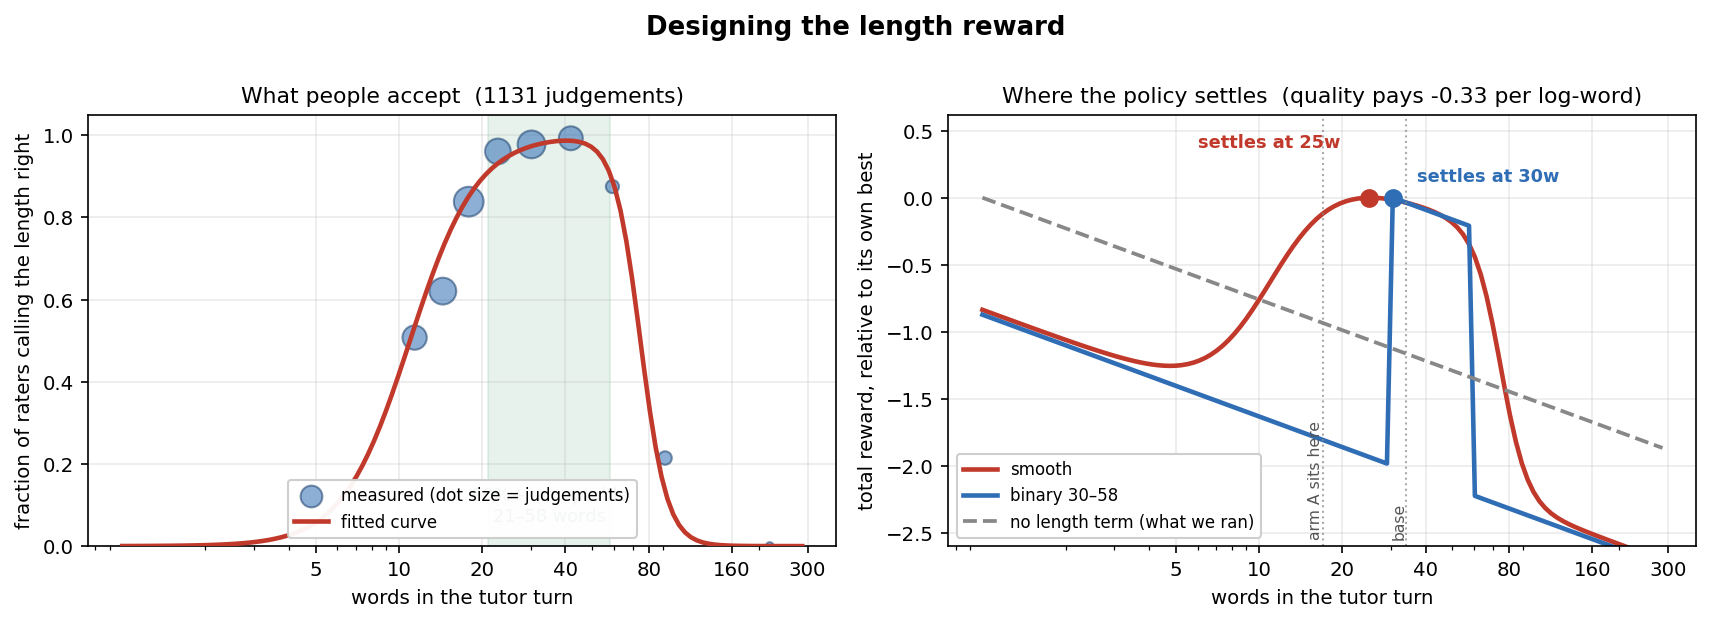
\includegraphics[width=\textwidth]{length_reward.png}
\caption{Left: acceptable lengths, from 1131 human judgements. Right: where the policy settles once the
probe's own pull toward brevity is accounted for. The band's interior is flat because that is what fixes
the resting length; a smooth peak drifts as the pull changes during training.}
\label{fig:lengthreward}
\end{figure}

\subsection{The learning-rate ladder}

Three runs at 2e-5, 4e-5 and 8e-5, identical otherwise --- same probe, same length term, same 200 steps.
This is the comparison arm B could not give, since z-scoring shrank its reward scale and thereby raised
its effective step size 3.4$\times$ as a side effect.

\begin{table}[h]
\centering
\begin{tabular}{llrrrrr}
\toprule
\textbf{Arm} & \textbf{Rate} & \shortstack{\textbf{Held-out}\\\textbf{reward}} & \textbf{Words} & \shortstack{\textbf{KL,}\\\textbf{final}}
& \shortstack{\textbf{KL,}\\\textbf{peak}} & \shortstack{\textbf{Steps to}\\\textbf{3.80}} \\
\midrule
E & 2e-5 & 3.84 & 27.2 & \textbf{0.25} & \textbf{0.31} & 133 \\
F & 4e-5 & \textbf{3.88} & 27.7 & 0.29 & 0.41 & 69 \\
G & 8e-5 & 3.86 & 28.2 & 0.29 & 0.41 & 65 \\
\bottomrule
\end{tabular}
\caption{Four times the learning rate buys 0.02 more reward and arrives twice as fast. Reward and length
are on held-out questions; KL is the mean over the last ten steps and its peak over the run; the last
column is the first step whose nine-step mean reaches 3.80.}
\label{tab:ladder}
\end{table}

All three converge to the same reward and the faster ones only arrive sooner --- a different answer from
the one the question presupposed. The reward is not a quantity a larger step can push higher: its ceiling
is what the probe can express, and all three optimisers reach it. Arm E's trajectory agrees: reward rose
3.13 $\rightarrow$ 3.84 over 200 steps, with successive 20-step gains of $+0.31$, $+0.14$, $+0.13$,
$+0.03$, $+0.02$, then eight increments of 0.03 or less.

\paragraph{The drift saturates rather than scaling with the rate.} 2e-5 $\rightarrow$ 4e-5 costs 0.04
nats; doubling again costs nothing, with F and G ending at the same 0.29 and peaking at the same 0.41.
Past 4e-5 the extra step size buys arrival time, not distance travelled, which makes 4e-5 better
supported than the 2e-5 the gain-per-KL measurement selected --- that ran 35 steps, before either arm had
converged.

\begin{figure}[h]
\centering
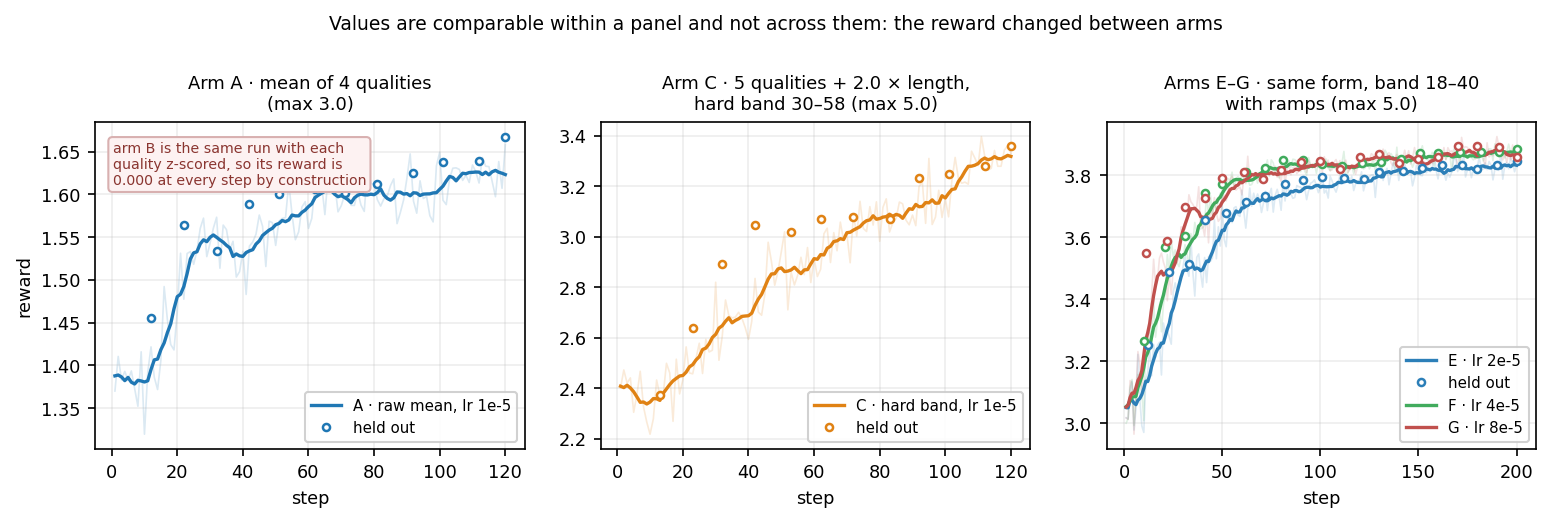
\includegraphics[width=\textwidth]{reward_all_arms.png}
\caption{Reward over training, one panel per reward \emph{definition}. Values are comparable within a
panel and not across them: arm A averages four qualities, arm C five plus a length term, and E--G use arm
C's form with a different band. Open circles are held-out questions, tracking the training curve
throughout.}
\label{fig:rewardall}
\end{figure}

\begin{figure}[h]
\centering
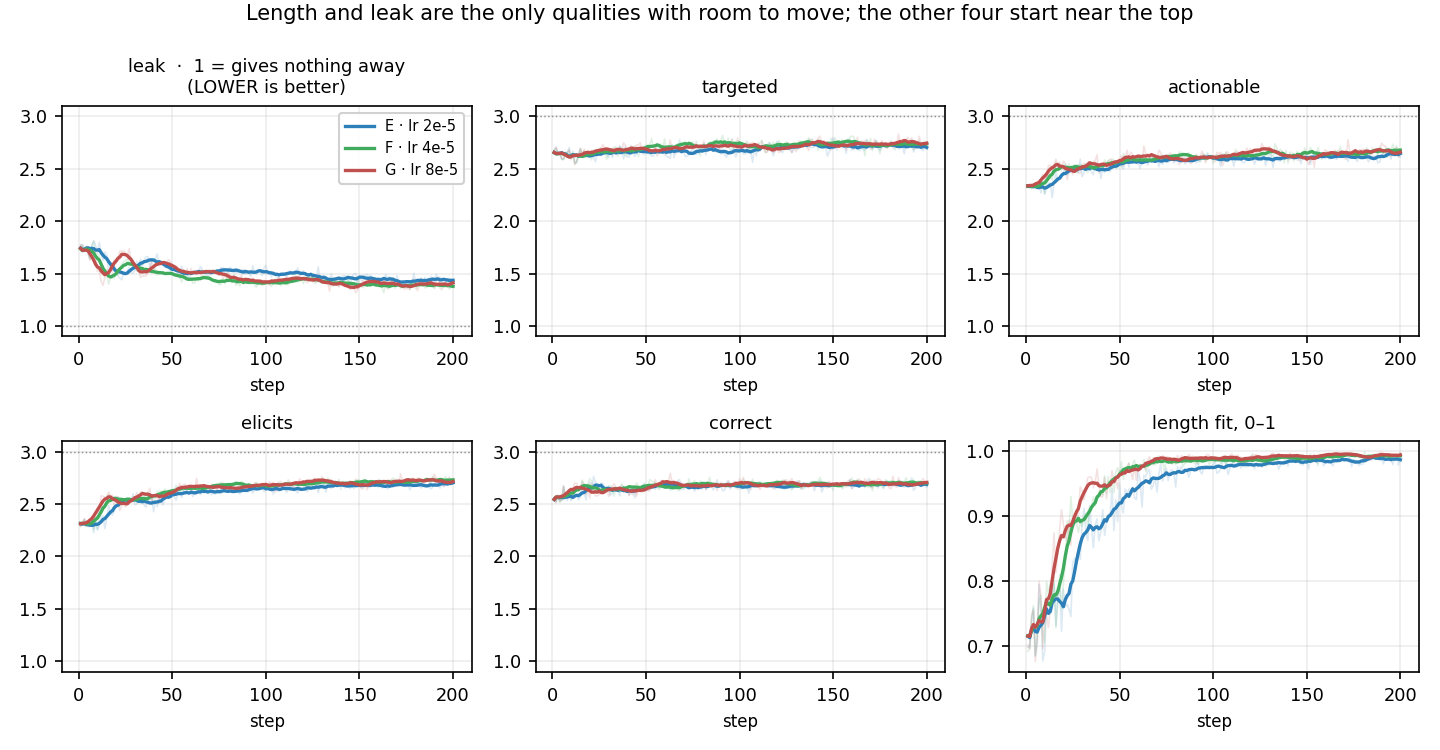
\includegraphics[width=\textwidth]{dimension_curves.png}
\caption{Which qualities actually moved. Only \qual{length} and \qual{leak} have real room:
\qual{targeted}, \qual{actionable}, \qual{elicits} and \qual{correct} start near 2.6 of 3 and finish
within 0.15 of where they began. This is Table~\ref{tab:ladder}'s ceiling seen per-quality.}
\label{fig:dimcurves}
\end{figure}

\begin{figure}[h]
\centering
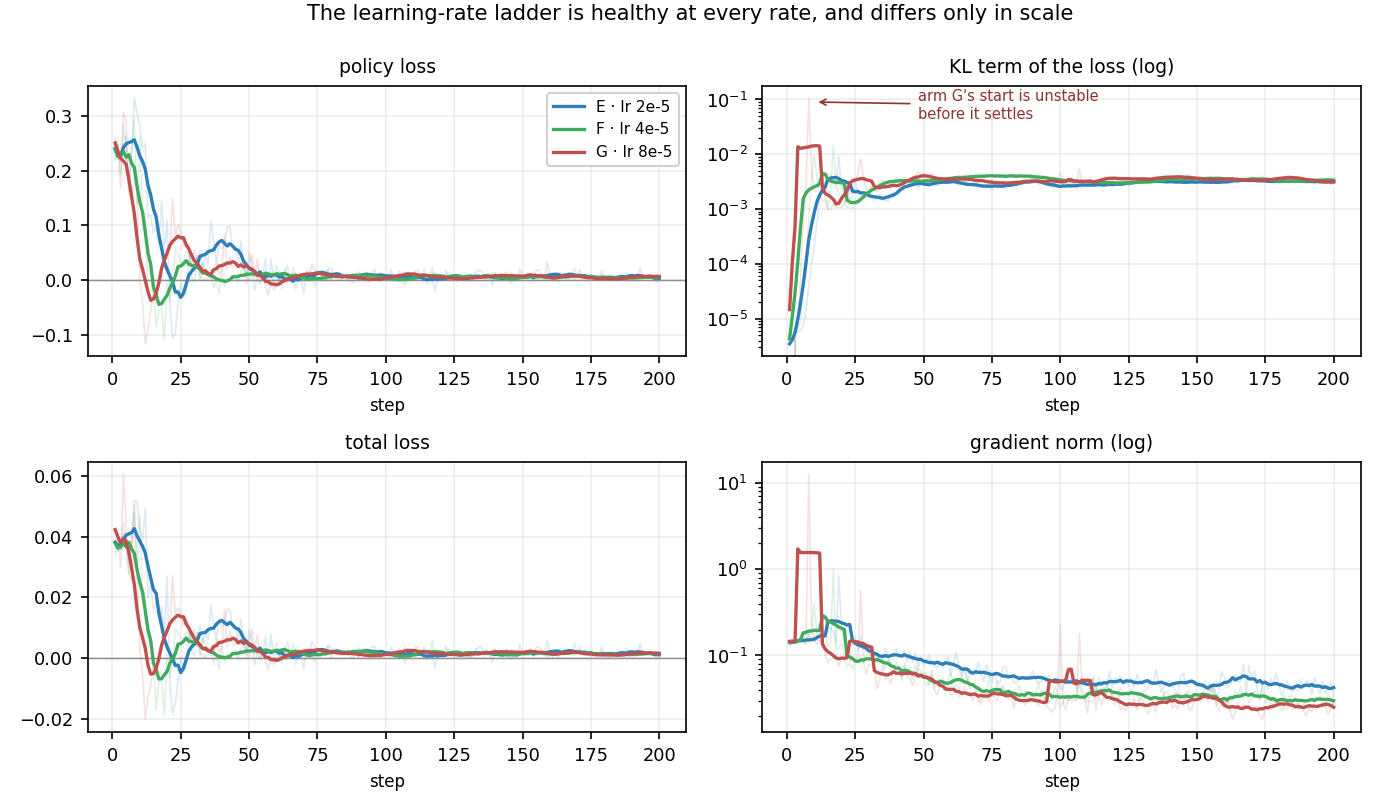
\includegraphics[width=\textwidth]{loss_curves.png}
\caption{Well-behaved at all three rates. Both right-hand panels are logarithmic because arm G spikes in
its first ten steps --- gradient norm 12.8 and KL term 0.106 against medians of 0.033 and 0.0034 --- the
only sign 8e-5 starts unstably before settling. Arm F's curve is stitched from three W\&B runs, since the
partition preempted it twice and each requeue resumed from the last checkpoint.}
\label{fig:losscurves}
\end{figure}

\begin{figure}[h]
\centering
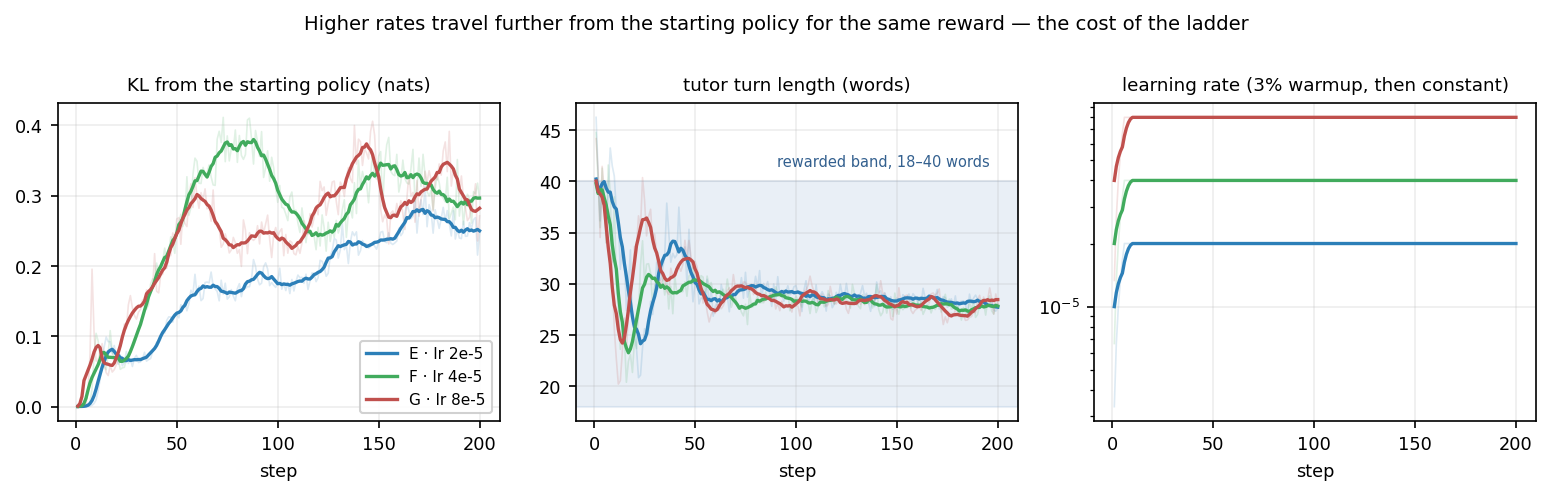
\includegraphics[width=\textwidth]{training_health.png}
\caption{Drift, generated length, and the schedule. Length falls \emph{into} the rewarded band and stops,
which is what the ramps were built to do and what arm C's hard band failed at. Four diagnostics are
constant and so not plotted: clipped tokens exactly 0, importance-ratio variance $10^{-15}$, mean
advantage $10^{-17}$, and no group of 16 samples ever scoring uniformly --- all consequences of strictly
on-policy single-epoch updates, where the importance ratio is 1 by construction.}
\label{fig:health}
\end{figure}

\paragraph{What this settles about arm B.} Arm B claimed $+0.49$ and was paid $+0.37$ at 3.4$\times$ arm
A's effective step size. Arms F and G are 2$\times$ and 4$\times$ arm E's and post the same reward, so arm
B's over-claiming was not a generic consequence of larger steps --- the scalarisation contributed something
step size alone does not. That question deserved, and never got, a test at matched step size.

\paragraph{Where the remaining headroom is.} Arm E ends at 3.84 against a maximum of 4.20. The length term
is saturated at 1.96 of 2.00 with 98\% of turns in band, while the five pedagogical qualities sit at 1.88
of 2.20. So roughly 85\% of what remains is in the qualities, and \qual{leak} is furthest from its ceiling
--- the same quality whose length coupling two repairs failed to remove.

\subsection{The ladder rated blind}

Sixty held-out questions answered by all four policies --- untrained plus three rates --- giving 240 turns,
blinded and rated by five calibrated models.

\begin{table}[h]
\centering
\begin{tabular}{lrrr}
\toprule
\textbf{Quality} & \textbf{E (2e-5)} & \textbf{F (4e-5)} & \textbf{G (8e-5)} \\
\midrule
\qual{elicits}     & $+0.48$ (73\%) & $+0.52$ (78\%) & $+0.49$ (75\%) \\
\qual{actionable}  & $+0.43$ (72\%) & $+0.41$ (66\%) & $+0.39$ (66\%) \\
\qual{leak}        & $+0.33$ (67\%) & $+0.32$ (70\%) & $+0.31$ (64\%) \\
\qual{correct}     & $+0.19$ (66\%) & $+0.17$ (68\%) & $+0.13$ (62\%) \\
\qual{length\_fit} & $+0.18$ (66\%) & $+0.18$ (67\%) & $+0.17$ (66\%) \\
\qual{targeted}    & $+0.14$ (69\%) & $+0.19$ (69\%) & $+0.13$ (68\%) \\
\midrule
\textbf{total}     & $\mathbf{+0.35}$ (80\%) & $\mathbf{+0.36}$ (86\%) & $\mathbf{+0.33}$ (80\%) \\
\bottomrule
\end{tabular}
\caption{Gain over untrained, paired by question. Percentages are the share of questions where the trained
turn was rated better. Every gain exceeds its margin of error.}
\label{tab:ladderblind}
\end{table}

\textbf{Every arm beats base on every quality}, which no earlier arm managed. Arm C won on four and lost
\qual{leak} because getting longer cost it there; arm E wins on all six, withholding more than base
\emph{while} being the right length --- unreachable earlier, when the only lever on length was a probe that
penalises it through \qual{leak}.

The length problem is closed: 100\% of turns rated right-length against base's 8\% / 82\% / 10\%. Arm C's
hard band left 29\% too short; moving the band to 18--40 words and adding ramps removed both tails.

\textbf{The three rates are interchangeable.} Totals of 1.73, 1.74 and 1.71, every quality within noise.
With reward converging to 3.84--3.88 and drift rising 0.25 $\rightarrow$ 0.29 then flattening, this is the
cleanest statement the project can make about the optimiser: it chooses how fast, the reward model chooses
how far.

\paragraph{Why this should not be believed yet.} These are model raters, and on arm C they were confidently
wrong: they tie leakage to length at $+0.59$ against the human's $+0.43$, and that bias made them rank arm
C below arm A when she preferred it 29--11. Arm E is \emph{shorter} than arm C, so the bias now runs in its
favour --- exactly when it should be trusted least. A blinded human preference test over 48 pairs is
outstanding and decides whether Table~\ref{tab:ladderblind} is a result or an artefact.

\subsection{All seven arms on one axis}

The reward changed definition four times, so no reward column compares all seven arms. But the four
\emph{original} qualities --- \qual{leak}, \qual{targeted}, \qual{actionable}, \qual{elicits} --- were
scored by the same four heads in every run, so their mean is comparable throughout.

\begin{table}[h]
\centering
\begin{tabular}{llrrrrl}
\toprule
\textbf{Arm} & \textbf{Rate} & \shortstack{\textbf{4-quality}\\\textbf{mean, start}}
& \shortstack{\textbf{4-quality}\\\textbf{mean, end}} & \textbf{Gain}
& \textbf{KL} & \textbf{Words} \\
\midrule
A & 1e-5 & 1.370 & 1.627 & $+0.257$ & 0.158 & 38 $\rightarrow$ 27 \\
B & 1e-5, z-scored & 1.388 & 1.724 & $+0.336$ & \textbf{0.567} & 43 $\rightarrow$ 23 \\
C & 1e-5, band 30--58 & 1.386 & 1.502 & $+0.116$ & 0.184 & 46 $\rightarrow$ 39 \\
D & 1e-5, ramps & --- & --- & --- & --- & --- \\
E & 2e-5, band 18--40 & 1.387 & 1.650 & $+0.263$ & 0.250 & 46 $\rightarrow$ 28 \\
F & 4e-5 & 1.382 & 1.685 & $+0.303$ & 0.293 & 45 $\rightarrow$ 28 \\
G & 8e-5 & 1.375 & 1.677 & $+0.302$ & 0.285 & 44 $\rightarrow$ 28 \\
\bottomrule
\end{tabular}
\caption{Every arm on the one quantity that never changed definition, averaged over the last ten steps as
scored by the probe --- what the probe believes, not what a human paid. Arm D is blank because the partition
preempted it at step 46, before its first checkpoint.}
\label{tab:allarms}
\end{table}

Two things only this table shows. \textbf{Arm B's drift was 3.6$\times$ arm A's} (0.567 against 0.158) at
the same nominal rate, which puts a number on the confound: z-scoring shrank the reward scale, and with
centred advantages that raises the effective step size rather than reweighting the qualities. Arm B was
never a test of scalarisation. And \textbf{arm C gained least of any completed arm} ($+0.116$ against
$+0.26$ to $+0.34$), because it spent its capacity getting longer --- the same trade that cost it
\qual{leak} and made the probe rank it below arm A while the human ranked it above.

\section{Capability Retention}
\label{sec:academic}
\claim{No detectable loss on ARC-Challenge, MMLU stem or GSM8K: $-0.3$ points pooled, bounded at $-1.5$.}

Everything so far compared tutoring against tutoring, but the policy was optimised for 200 steps against a
reward built entirely from the shape of a turn, which says nothing about whether it can still do arithmetic
or recall a fact --- and narrow objectives are documented to cost capability elsewhere.

So both trained arms and base were asked to \emph{answer} rather than teach, on three benchmarks none of
them trained on. Multiple-choice items are scored by the loglikelihood assigned to each option letter,
which avoids depending on format compliance; GSM8K is generated and the final number parsed. Every arm sees
an identical 400 items per benchmark, decoding is greedy, and differences use McNemar's exact test on the
items where two models disagree.

\begin{table}[h]
\centering
\begin{tabular}{lccc}
\toprule
& base & arm E (2e-5) & arm G (8e-5) \\
\midrule
ARC-Challenge & 70.8\% & 70.8\% & 70.8\% \\
MMLU stem & 42.5\% & 42.0\% & 42.0\% \\
GSM8K & 83.8\% & 83.2\% & 83.0\% \\
\midrule
pooled change & --- & $-0.3$ [$-1.1$, $+0.5$] & $-0.4$ [$-1.5$, $+0.7$] \\
\bottomrule
\end{tabular}
\caption{Capability is unchanged. Pooled change is the paired difference over all 1200 items in percentage
points, with a 95\% interval; $p=0.54$ and $p=0.56$.}
\label{tab:academic}
\end{table}

\begin{figure}[h]
\centering
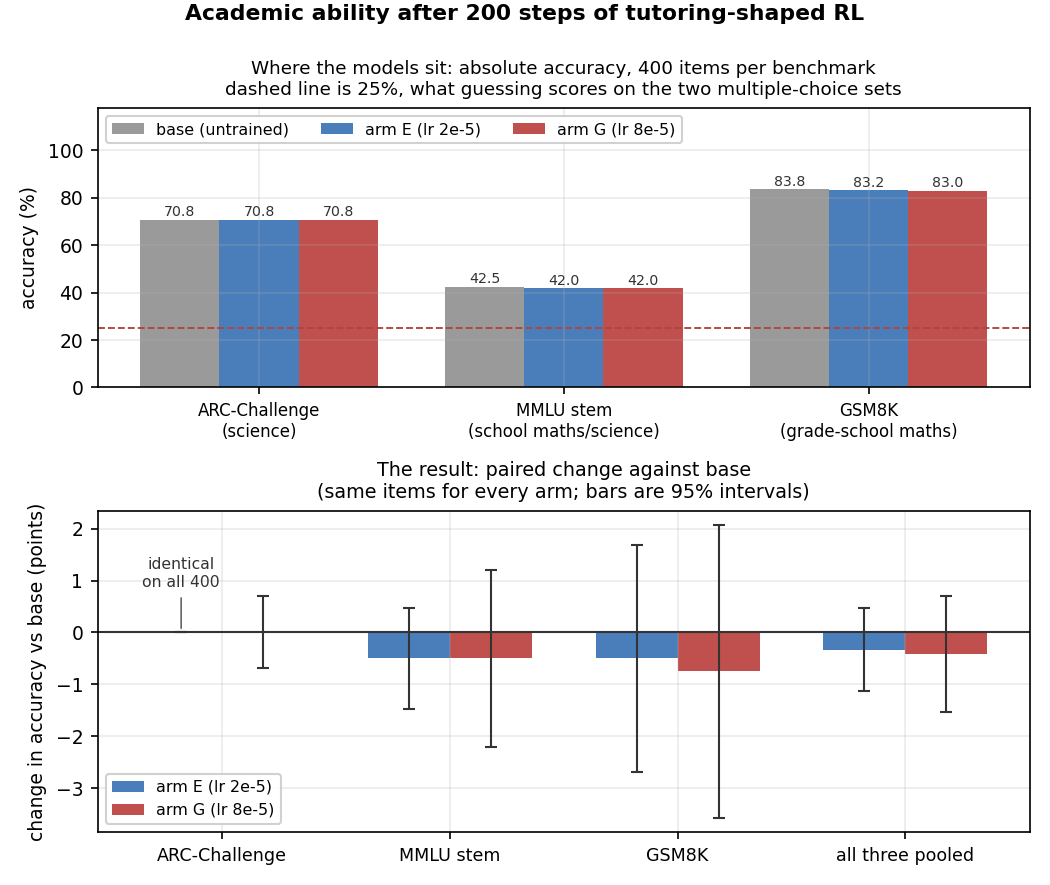
\includegraphics[width=0.92\textwidth]{academic_ability.png}
\caption{Top: absolute accuracy, which situates the result --- MMLU stem at 42.5\% is close enough to the
25\% chance floor that little of the scale is in play, while GSM8K at 83.8\% has little headroom, and a
0.3-point change means something different in each case. Bottom: the paired difference, plotted separately
because at 42\% and 84\% the raw bars are visually identical whatever the gap.}
\label{fig:academic}
\end{figure}

\paragraph{Nothing moved.} Pooled over 1200 items, arm E is 0.3 points below base and arm G 0.4, both
inside noise. On ARC-Challenge arm E is not merely equal to base but identical item for item: none of the
400 changed hands.

\paragraph{The null is bounded, not merely unrefuted.} This matters more than the $p$-value, since ``we
observed no change'' and ``we could not have observed a change'' read identically. Pooled, we exclude any
drop worse than roughly 1.5 points. Per benchmark the intervals are much wider --- GSM8K's reaches $-3.6$
--- which is why the pooled figure carries the claim. It is also the expected outcome: arm E ends at 0.25
nats, and a rank-32 adapter over a frozen 7B has limited capacity to overwrite what the base knows. Had
capability fallen anyway, the tutoring gains would have been paid for out of something else.

\paragraph{Two harness faults preceded these numbers, both giving confident wrong answers.} Generation was
first capped at 24 tokens, on the assumption a direct question draws a direct answer; instruction-tuned
models reason first, so half the GSM8K generations were truncated mid-derivation and measured accuracy came
out at 1.8\% against a published $\sim$67\%. Raising the budget to 512 still left 30\% of MMLU items
unparseable --- and that failure is correlated with the quantity under test, since a more verbose policy
loses more items to truncation. Under that harness arm G appeared to fall 41.0\% $\rightarrow$ 36.2\%,
where option loglikelihoods give 42.5\% against 42.0\%. A parse-failure rate that differs across arms is
not noise but a bias with a sign, and it pointed toward concluding the trained models were worse.

\section{Limitations}
\label{sec:limits}

\begin{itemize}
\item \textbf{Questions were held out from the policy but not from the probe.} The 250 training and 50
evaluation questions do not overlap, but 45 of the 50 were among those the probe was fitted on. Nothing
leaks, since the probe is frozen, but any agreement measured here flatters it.
\item \textbf{One human, 17 questions rated and 28 pairs decided.} Every claim about which policy is better
rests on 60 questions rated by models whose per-turn agreement with her is weak, plus her own 17. They
agree, which is why either is believable, but neither is a large sample.
\item \textbf{Only the final checkpoint was evaluated.} Checkpoints exist every 10 steps, so if quality
peaked earlier while reward kept climbing, this would not show it.
\item \textbf{The probe reads text far from what it was fitted on.} The encoder is frozen, but it was fitted
on base-model turns and by step 200 reads policy text at 0.25 nats and 28 words against 46. That shift
defeated both \qual{leak} repairs.
\item \textbf{Why nobody agrees per turn on \qual{elicits} and \qual{actionable} is unexplained.} Both are
near-saturated here, so what remains may be taste rather than a learnable signal.
\end{itemize}

\section{Conclusion}
\label{sec:conclusion}

A ridge fit on a frozen model's activations is a usable RL reward for tutoring quality, and its claimed
improvement held up under a blind check by raters who could not see it --- which the predecessor
outcome-based reward conspicuously failed. It is not a fine instrument: it cannot separate two policies that
have both climbed it, and optimising it harder produced a policy that claimed more than it was paid.

What we did not expect is that optimising it would be the easy part. Three learning rates spanning
4$\times$ reach the same place, four of six qualities sit near their ceiling before training starts, and the
one quality with real headroom is the one whose length coupling resisted two principled repairs. The
optimiser was never the constraint. Three things follow:

\begin{enumerate}
\item \textbf{Collect labels on policy-generated turns.} The $+0.70$ length coupling exists only out of
distribution, so no correction estimated on the existing corpus reaches it. This is the highest-value
annotation left and it unblocks the only quality with headroom.
\item \textbf{Use 4e-5, not 2e-5.} Same reward in half the steps at the same final drift. The gain-per-KL
measurement that chose 2e-5 ran 35 steps, before either arm converged.
\item \textbf{Evaluate intermediate checkpoints.} If quality peaks before reward does, that is where to
stop, and locating it beats a run that happened to stop early.
\end{enumerate}

\end{document}
